%%%%%%%%%%%%%%%%%%%%%%%%%%%%%%%%%%%%%%%%%%%%%%%%%%%%%%%%%%%%%%%%%%%%%%%%%%
%                                                                        %
%  The Why platform for program certification                            %
%                                                                        %
%  Copyright (C) 2002-2011                                               %
%                                                                        %
%    Jean-Christophe FILLIATRE, CNRS & Univ. Paris-sud 11                %
%    Claude MARCHE, INRIA & Univ. Paris-sud 11                           %
%    Yannick MOY, Univ. Paris-sud 11                                     %
%    Romain BARDOU, Univ. Paris-sud 11                                   %
%                                                                        %
%  Secondary contributors:                                               %
%                                                                        %
%    Thierry HUBERT, Univ. Paris-sud 11  (former Caduceus front-end)     %
%    Nicolas ROUSSET, Univ. Paris-sud 11 (on Jessie & Krakatoa)          %
%    Ali AYAD, CNRS & CEA Saclay         (floating-point support)        %
%    Sylvie BOLDO, INRIA                 (floating-point support)        %
%    Jean-Francois COUCHOT, INRIA        (sort encodings, hyps pruning)  %
%    Mehdi DOGGUY, Univ. Paris-sud 11    (Why GUI)                       %
%                                                                        %
%  This software is free software; you can redistribute it and/or        %
%  modify it under the terms of the GNU Lesser General Public            %
%  License version 2.1, with the special exception on linking            %
%  described in file LICENSE.                                            %
%                                                                        %
%  This software is distributed in the hope that it will be useful,      %
%  but WITHOUT ANY WARRANTY; without even the implied warranty of        %
%  MERCHANTABILITY or FITNESS FOR A PARTICULAR PURPOSE.                  %
%                                                                        %
%%%%%%%%%%%%%%%%%%%%%%%%%%%%%%%%%%%%%%%%%%%%%%%%%%%%%%%%%%%%%%%%%%%%%%%%%%

\documentclass[a4paper,11pt,twoside,openright]{report}

\usepackage[a4paper=true,pdftex,colorlinks=true,urlcolor=blue,pdfstartview=FitH]{hyperref}

\usepackage[latin1]{inputenc}
\usepackage[T1]{fontenc}
\usepackage{times}
\usepackage{amssymb}
\usepackage{graphicx}
%\usepackage{color}
%\usepackage{mathptm}
%\usepackage{xspace}
\usepackage{makeidx}
\makeindex
\input{./version.tex}

% common Why title page

\newcommand{\whytitlepage}[4]{%
\begin{titlepage}
\begin{center}
~\vfill
\rule\textwidth{0.1cm}\\[0.5cm]
\begin{Huge}\sffamily
#1 % title
\end{Huge}
\\[1cm]
\begin{Large}\sffamily
#2
\end{Large}
\\[0.1cm]
\rule\textwidth{0.1cm}\\[1cm]
Version #3\\[3cm]
#4
\vfill
\today\\
INRIA Team-Project \emph{Proval} \url{http://proval.lri.fr} \\
INRIA Futurs \& LRI, CNRS UMR 8623\\ 
4, rue Jacques Monod, 91893 Orsay cedex, France
\end{center}
\end{titlepage}}

\newcommand{\why}{\textsf{Why}}
\newcommand{\Why}{\why}
\newcommand{\java}{\textsc{Java}\index{Java@\textsf{Java}}}
\newcommand{\Java}{\java}
\newcommand{\krakatoa}{\textsf{Krakatoa}\index{Krakatoa@\textsf{Krakatoa}}}
\newcommand{\Krakatoa}{\krakatoa}
\newcommand{\caduceus}{\textsf{Caduceus}\index{Caduceus@\textsf{Caduceus}}}
\newcommand{\Caduceus}{\caduceus}
\newcommand{\coq}{\textsf{Coq}\index{Coq@\textsf{Coq}}}
\newcommand{\Coq}{\coq}
\newcommand{\pvs}{\textsf{PVS}\index{PVS@\textsf{PVS}}}

%

\newcommand{\kw}[1]{\ensuremath{\mathsf{#1}}}

% types
\newcommand{\bool}{\kw{bool}}
\newcommand{\unit}{\kw{unit}}
%\newcommand{\tref}[1]{\ensuremath{#1~\kw{ref}}}
\newcommand{\tref}[1]{\ensuremath{#1~\mathsf{ref}}}
\newcommand{\tarray}[2]{\ensuremath{\kw{array}~#1~\kw{of}~#2}}

% constructs
\newcommand{\prepost}[3]{\ensuremath{\{#1\}\,#2\,\{#3\}}}
\newcommand{\result}{\ensuremath{\mathit{result}}}

\newcommand{\void}{\kw{void}}
\newcommand{\access}[1]{\ensuremath{!#1}}
\newcommand{\assign}[2]{\ensuremath{#1~:=~#2}}
\newcommand{\pref}[1]{\ensuremath{\kw{ref}~#1}}
\newcommand{\taccess}[2]{\ensuremath{#1\texttt{[}#2\texttt{]}}}
\newcommand{\tassign}[3]{\ensuremath{#1\texttt{[}#2\texttt{]}~\texttt{:=}~#3}}
\newcommand{\faccess}[2]{\ensuremath{(\mathit{access}~#1~#2)}}
\newcommand{\fupdate}[3]{\ensuremath{(\mathit{update}~#1~#2~#3)}}
%\newcommand{\taccess}[2]{\ensuremath{#1[#2]}}
%\newcommand{\tassign}[3]{\ensuremath{#1[#2]~:=~#3}}
%\newcommand{\faccess}[2]{\ensuremath{(\mathit{access}~#1~#2)}}
%\newcommand{\fupdate}[3]{\ensuremath{(\mathit{update}~#1~#2~#3)}}
% \newcommand{\block}[1]{\ensuremath{\kw{begin}~#1~\kw{end}}}
\newcommand{\seq}[2]{\ensuremath{#1;~#2}}
%\newcommand{\plabel}[2]{\ensuremath{#1:#2}}
\newcommand{\plabel}[2]{\ensuremath{#1\texttt{:}#2}}
\newcommand{\assert}[2]{\ensuremath{\kw{assert}~\{#1\};~#2}}
\newcommand{\while}[4]{\ensuremath{\kw{while}~#1~\kw{do}~\{\kw{invariant}~#2~\kw{variant}~#3\}~#4~\kw{done}}}
\newcommand{\ite}[3]{\ensuremath{\kw{if}~#1~\kw{then}~#2~\kw{else}~#3}}
\newcommand{\fun}[3]{\ensuremath{\kw{fun}~#1:#2\rightarrow#3}}
\newcommand{\app}[2]{\ensuremath{(#1~#2)}}
\newcommand{\rec}[4]{\ensuremath{\kw{rec}~#1:#2~\{\kw{variant}~#3\}=#4}}
\newcommand{\letin}[3]{\ensuremath{\kw{let}~#1=#2~\kw{in}~#3}}
\newcommand{\raisex}[2]{\ensuremath{\kw{raise}~(#1~#2)}}
\newcommand{\exn}[1]{\ensuremath{\kw{Exn}~#1}}
\newcommand{\try}[2]{\ensuremath{\kw{try}~#1~\kw{with}~#2~\kw{end}}}
\newcommand{\coerce}[2]{\ensuremath{(#1:#2)}}

\newcommand{\statement}{\textit{statement}}
\newcommand{\program}{\textit{program}}
\newcommand{\expression}{\textit{expression}}
\newcommand{\predicate}{\textit{predicate}}

% inference rules
\newcommand{\espacev}{\rule{0in}{1em}}
\newcommand{\espacevn}{\rule[-0.4em]{0in}{1em}}
\newcommand{\irule}[2]
  {\frac{\espacevn\displaystyle#1}{\espacev\displaystyle#2}}
\newcommand{\typage}[3]{#1 \, \vdash \, #2 : #3}
\newcommand{\iname}[1]{\textsf{#1}}

\newcommand{\emptyef}{\bot}
\newcommand{\wf}[1]{#1~\kw{wf}}
\newcommand{\pur}[1]{#1~\kw{pure}}
\newcommand{\variant}[1]{#1~\kw{variant}}

\newcommand{\wpre}[2]{\ensuremath{\mathit{wp}(#1,#2)}}
\newcommand{\wprx}[3]{\ensuremath{\mathit{wp}(#1,#2,#3)}}

\newcommand{\barre}[1]{\ensuremath{\overline{#1}}}

%%% Local Variables: 
%%% mode: latex
%%% TeX-master: "doc"
%%% End: 


\setlength{\textheight}{240mm}
\setlength{\topmargin}{-10mm}
\setlength{\textwidth}{160mm}
\setlength{\oddsidemargin}{0mm}
\setlength{\evensidemargin}{0mm}

\renewcommand{\textfraction}{0.01}
\renewcommand{\topfraction}{0.99}
\renewcommand{\bottomfraction}{0.99}

\usepackage{fancyhdr}
\pagestyle{fancyplain}
\renewcommand{\footrulewidth}{0.4pt}
\addtolength{\headheight}{2pt}
\addtolength{\headwidth}{1cm}
\renewcommand{\chaptermark}[1]{\markboth{#1}{}}
\renewcommand{\sectionmark}[1]{\markright{\thesection\ #1}}
\lhead[\fancyplain{}{\bfseries\thepage}]{\fancyplain{}{\bfseries\rightmark}}
\chead{}
\rhead[\fancyplain{}{\bfseries\leftmark}]{\fancyplain{}{\bfseries\thepage}}
\lfoot{\fancyplain{}{ProVal}}
\cfoot{\fancyplain{}{Why platform}}
\rfoot{\fancyplain{}{\today}}


\begin{document}
\sloppy
\hbadness=9999

\whytitlepage{The Why Platform \\~\\for Program Verification}{Main Documentation}{1.0}{Jean-Christophe Filli\^atre, Claude March\'e}


\tableofcontents

\chapter{Introduction}

Why/Krakatoa/Caduceus is a set of tools for deductive verification of
Java and C source code. In both cases, the requirements are specified
as \emph{annotations} in the source, in a special style of comments.
For Java (and Java Card), these specifications are given in the
\emph{Java Modeling Language}~\cite{Burdy04} and are interpreted by
the \emph{Krakatoa} tool. For C, we designed our own specification
language, largely inspired from JML. Those are interpreted by the
\emph{Caduceus} tool. The tools are available as open source software
at \url{http://why.lri.fr/}. 

\begin{figure}
\begin{center}
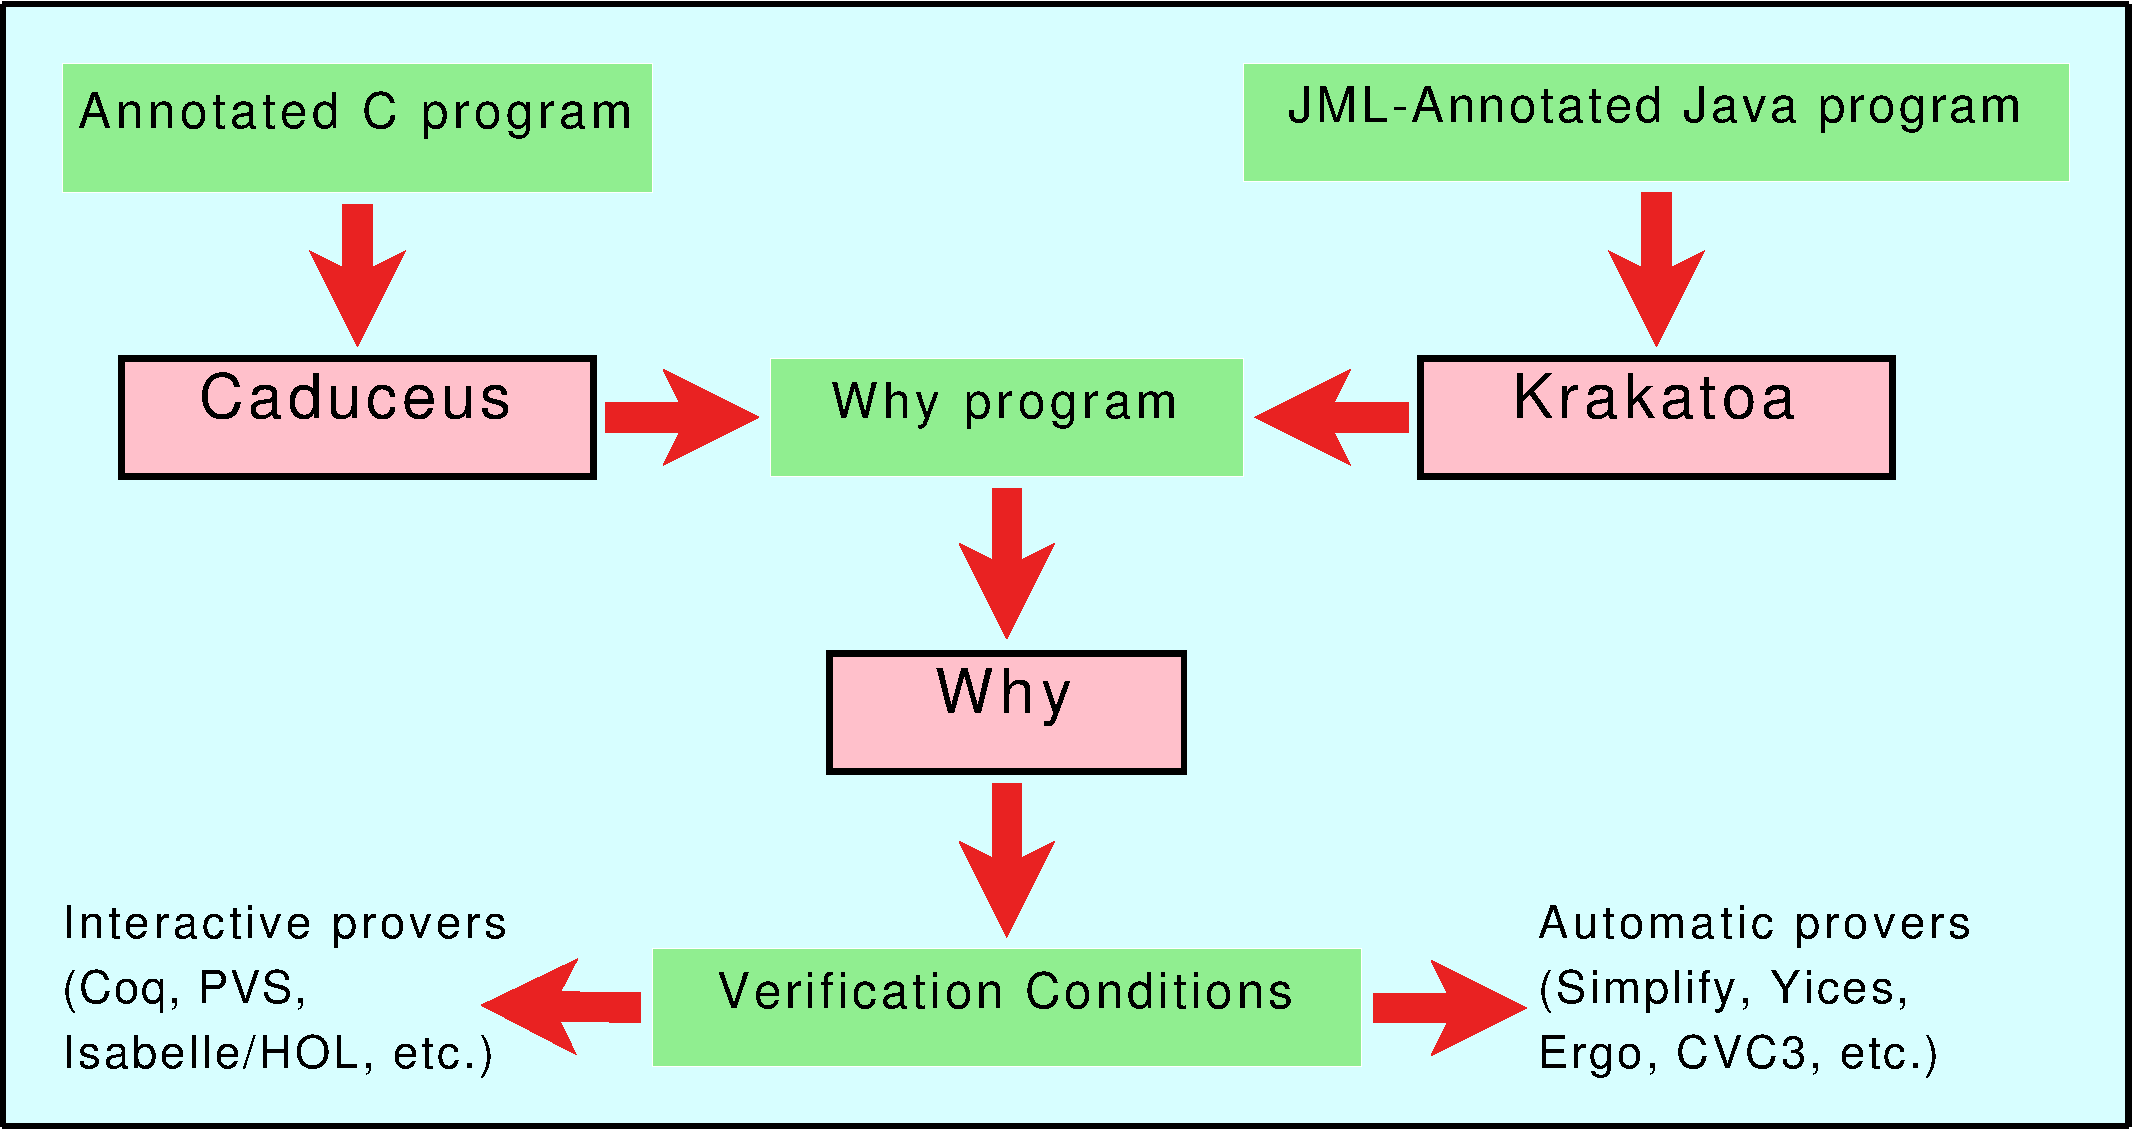
\includegraphics[width=\textwidth]{platform2.pdf}
\end{center}
\caption{Platform Architecture\label{fig:arch}}
\end{figure}

The overall architecture is presented on Figure~\ref{fig:arch}. The
general approach is to generate \emph{Verification Conditions} (VCs
for short): logical formulas whose validity implies the soundness of
the code with respect to the given specification.  This includes
automatically generated VCs to guarantee the absence of run-time
errors: null pointer dereferencing, out-of-bounds array access, etc.
Then the VCs can be discharged using one or several theorem provers.
The main originality of this platform is that a large part is common
to C and Java. In particular there is a unique, stand-alone, VCs
generator called Why, which is able to output VCs in the native syntax
of many provers, either automatic or interactive ones.


You will find specific documentation for tools in the following documents:
\begin{itemize}
\item The \Why{} language and VCG: Reference Manual: \texttt{manual.ps} 
\item \Krakatoa{} for Java verification: Tutorial and Reference Manual: \texttt{krakatoa.pdf} 
\item \Caduceus{} for C verification: Tutorial and Reference Manual: \texttt{caduceus.ps} 
\end{itemize}


In the next chapter you will find various additional informations,
including the requirements, a summary of known limitations, and how to
get help. 


\chapter{Technical notes}

\section{Requirements}
\label{app:requirements}

NEED UPDATE

User requirements: knowing how to perform proofs using the Coq
system. Knowing how to write JML specifications.

System requirements: \Coq{} version 8.0, \Why{} version 1.32 or higher. For
compiling \Krakatoa{} from sources, you need also the Objective Caml
compiler, version 3.04 or higher.

\section{Installation procedure}

\subsection{From the sources}

Get a copy of sources at the web page \url{http://why.lri.fr/}. 

Decompress the archive in a directory of your choice.

Run commands
\begin{verbatim}
./configure
make
make install
\end{verbatim}

\subsection{Binaries}

Please look at the web page \url{http://why.lri.fr/} for binaries for
popular architectures. Krakatoa is distributed as part of the Why
debian package, available on standard repositories of debian-based
distributions.
 
\section{Summary of features and known limitations}
\label{sec:features}

TODO: this is only Krakatoa

\begin{itemize}
%\item No checking of arithmetic overflow

\item Unsupported kind of statements in translation: ...

\item exception NullPointerException and ArrayOutOfBoundsException are
required NOT to be thrown, and consequently should not be catched.

%\item Method parameters are not modifiable.

\item For recursive or mutually recursive methods, only partial
correctness is guaranteed.

%\item some valid Java identifiers should not be used in your programs,
%  unless some name clashes may occur: identifiers starting by
%  \verb|krak| ;
%  names introduced in the generated model: \verb|access|,
%  \verb|update|, etc. ; keywords of \Why: result, parameter, etc.
\end{itemize}

\section{Contacts}

The web page for the Why platform is at URL \url{http://why.lri.fr/}.

For general questions regarding the use of the platform tools, please
use the Why mailing list. You need to subscribe to the list before
sending a message to it. To subscribe, follow the instructions given
on page
\url{http://lists.gforge.inria.fr/cgi-bin/mailman/listinfo/why-discuss}

For bug reports, please use the bug tracking system at
\url{https://gforge.inria.fr/tracker/?atid=4012&group_id=999&func=browse}. For
security reasons, you need to register before submitting a new
bug. Please create an account there, where you can put "ProVal" for
the required field "INRIA Research Project you work with or work in".

In case if the mailing list above is not appropriate, you can contact
the authors directly at the following address: \url{mailto:Jean-Christophe dot
  Filliatre at lri dot fr}.\url{mailto:Claude dot
  Marche at inria dot fr}.

\cleardoublepage

\addcontentsline{toc}{chapter}{\bibname}
\bibliographystyle{plain}
\bibliography{./biblio}
\cleardoublepage

\addcontentsline{toc}{chapter}{\indexname}
\printindex
\cleardoublepage

\end{document}

%%% Local Variables:
%%% mode: latex
%%% TeX-PDF-mode: t
%%% TeX-master: t
%%% End:
